\chapter{Correttezza di programmi sequenziali}
\label{Capitolo 3}
Introduciamo l'argomento con un esempio.
\begin{esempio}
	Definiamo una funzione in C che riceve un vettore, un intero (la lunghezza del vettore) e
	e restituisce un ulteriore numero intero.
	\begin{listing}[ht]
		\begin{minted}{c}
			int f(int n, const int v[]) {
				int x = v[0];
				int h = 1;
				while (h < n) {
					if (x < v[h])
					x = v[h];        
					h = h + 1;
				}
				return x;
			}
		\end{minted}
		\caption{Esempio di funzione in C}
		\label{listing:1}
	\end{listing}
	La funzione scopriamo che si occupa di cercare il massimo in
	un vettore: la strategia della funzione è quella di spostarsi lungo il vettore e
	conservare in $x$ il valore massimo fino a ora trovato. Arrivati alla fine
	del vettore so che in $x$ avrò il valore massimo.\\
	Fissiamo le \textbf{condizioni iniziali}: più formalmente suppongo che $n$ sia $n > 0$, per dire che abbiamo almeno un
	elemento nel vettore. Suppongo inoltre che $v[i]\in\mathbb{Z},\,\,\forall i\in
	\{0,\ldots, n-1\}$. \\
	All'inizio $x$ è il massimo del sotto-vettore con solo il primo elemento
	($v[0]$) e dopo l'assegnamento di $h$ in $v[0..h-1]$, che, con $h=1$ mi
	conferma che x è il massimo in $v[0..0]$. \\
	\begin{nota}
	Indichiamo con $v[0..n]$ l'insieme $\{v[0] \dots v[n]\}$ 
	\end{nota}
	Al termine di una certa iterazione $x$ contiene il massimo 
	tra i valori compresi tra $v[0]$ e $v[h-1]$ (detto altrimenti il massimo in
	$v[0..h-1]$). Inoltre al fine di una certa iterazione ci aspetto che $h\leq
	n$.\\
	Possiamo quindi dire che quando esco dal ciclo $x$ è il massimo in $v[0..h-1]$
	ma in questo momento $h=n$ e quindi $x$ è il massimo del vettore.\\
	Consideriamo ora la parte iterativa. All'inizio di ogni iterazione suppongo
	che $x$ è il massimo in $v[0..h-1]$. Dopo l'istruzione di scelta $x$ è il
	massimo in $v[0..h]$, comunque sia andata la scelta. Alla fine
	dell'iterazione, dopo l'incremento di $h$, avrò ancora che $x$ è il massimo in
	$v[0..h-1]$. ragioniamo quindi per induzione. Se all'inizio dell'iterazione e
	alla fine abbiamo la stessa asserzione, ed è vera prima d'iniziare l'iterazione,
	posso dire che abbiamo una \textbf{proprietà invariante} e vale anche al termine
	dell'ultima iterazione e quindi vale anche alla fine dell'esecuzione del
	programma. 
\end{esempio}
\begin{definizione}[Invariante - Prima definizione]
    Relazione, tra i valori delle variabili del programma, che ha questa caratteristica: se vale all'inizio di una certa iterazione allora varrà, indipendentemente dal cambiamento di valore delle variabili, anche al termine dell'iterazione.
\end{definizione}
Nell'esempio notiamo l'assenza di formalità. Si introducono quindi
concetti:
\begin{enumerate}
	\item \textbf{pre-condizione} che nell'esempio è fatta da $n>0$ e
	      $v[i]\in\mathbb{Z},\,\,\forall i\in \{0,\ldots, n-1\}$
	\item \textbf{post-condizione} che nell'esempio si ritrova con l'asserzione $x$
	      è il massimo in $v[0..h-1]$ e $h=n$, che scritto in modo formale diventa:
	      \[
	      	\begin{rcases}
	      		v[i]\leq x,\,\,\forall i\in \{0,\ldots, n-1\}\\
	      		\exists\, i\in\{0,\ldots, n-1\}\mbox{ t.c. } v[i]=x
	      	\end{rcases}
	      	x=max(v[0..n-1])
	      \]
\end{enumerate}
\textit{Queste formule possono essere rese come formule proposizionali, tramite
una congiunzione logica:}
\[
	\begin{cases}
		v[0]\leq x \land v[1]\leq x\land\ldots v[n-1]\leq x \\
		v[0]= x \lor v[1]= x\lor\ldots v[n-1]=x             
	\end{cases}
\]
Abbiamo studiato lo stato della memoria del programma in un certo istante
tramite formule.
\begin{definizione}
	Definiamo \textbf{stato della memoria} come:
	\[s:V\to\mathbb{Z}\]
	ovvero una funzione che mappa le variabili del programma (poste nell'insieme
	$V$) in $\mathbb{Z}$.
\end{definizione} \vspace{5mm} %5mm vertical space
Fissato uno stato della memoria e una formula posso validare una formula in
quello stato osservando le variabili e le relazioni aritmetiche della
formula.\\
Data una formula $\phi$ e uno stato $s$ posso sapere se $\phi$ è valida in
$s$.\\
Una formula che gode della \textbf{proprietà invariante} se è vera all'inizio
dell'iterazione è vera anche alla fine della stessa. Per capire se è invariante
basta vedere lo stato di una formula ad inizio e fine di una iterazione.\\
L'esecuzione di una istruzione cambia lo stato della memoria. Potrebbe però
accadere che una serie di istruzioni non facciano terminare il programma, perciò
quanto detto sopra è in realtà un'approssimazione della realtà.
\begin{definizione}
	Definiamo la \textbf{specifica di correttezza di un programma} con la tripla:
	\[\alpha\,\, P\,\, \beta\]
	dove:
	\begin{itemize}
		\item $\alpha$ e $\beta$ sono formule (definite con tutte le simbologie
		      aritmetiche tra variabili, sia di conto che di relazione).
		\item $P$ è un ``programma'' (anche un frammento o una singola istruzione) che
		      modifica lo stato della memoria.
	\end{itemize}
	$\alpha$ è la \textbf{pre-condizione}, che supponiamo verificata nello stato
	iniziale e $\beta$ è la \textbf{post-condizione}, 
	che supponiamo valida dopo l'esecuzione del programma.
\end{definizione} \vspace{5mm} %5mm vertical space
Durante il corso useremo un linguaggio imperativo non reale semplificato.
Dovremo anche definire una logica, definendo un apparato deduttivo, un insieme
di regole per costruire dimostrazioni derivando nuove formule da quelle
preesistenti. Useremo la \textbf{logica di Hoare}. Le formule della logica di
Hoare sono triple di tipo $(\alpha P \beta)$ quindi si tratta di una logica di tipo diverso
anche se si appoggia su quella proposizionale.
\section{Linguaggio semplificato}
Definiamo quindi il linguaggio di programmazione imperativo semplificato che
andremo a utilizzare. Si userà una grammatica formale.\\
L'elemento fondamentale di questo linguaggio è il \textbf{comando}, che indica o
una singola istruzione o un gruppo d'istruzioni strutturate. Il simbolo usato
nella grammatica per indicare un comando è ``C''. Un comando viene costruito
tramite le \textbf{produzioni}, introdotte da ``::=''. Il comando più semplice è
l'\textbf{assegnamento}, che usa l'operatore ``:='' per assegnare un valore ad
una variabile. Con il simbolo ``è' indichiamo un simbolo non terminale della
grammatica che sta per \textit{espressione}. Una volta costruito semplici
espressioni possiamo combinarle, eseguendole in sequenza, inserendo un ``;'' tra
due comandi.\\ 
In merito all'istruzione di scelta abbiamo l'istruzione ``if'', seguito da
un'espressione booleana, seguito da ``then'', seguita da un comando, seguita da
``elsè', seguita da un comando, e il tutto viene concluso da ``endif''. Qui
abbiamo una prima semplificazioni dicendo che l'\textit{else} è
obbligatorio. Per l'iterazione abbiamo il ``whilè', seguito da un'espressione
booleana, seguito da ``do'' con poi il comando, il tutto concluso da
endwhile. Infine abbiamo una istruzione speciale, chiamata ``skip'', che non fa
nulla e avanza il \textit{program counter} (con essa posso saltare il ramo
alternativo dell'\textit{if-else}).\\
Un'espressione booleana ``B'' può essere la costante ``truè', la costante
``falsè' o del tipo ``not B'', ``B and B'', ``B or B'', ``E < è' (e le altre),
``E = è'. Non si hanno tipi di dato ma supporremo di avere a che fare solo con
\textit{interi}. Non si ha la funzione di nozione o di classe. Questo linguaggio
è comunque \textit{Turing Complete}.
\begin{listing}[H]
	\begin{lstlisting}
    x ~ a; y ~ b;
    while x != y do
      if x < y then
        y ~ y - x;
      else
        x ~ x - y;
      endif
    endwhile  
	\end{lstlisting}
	\caption{Esempio di programma $D$}
	\label{listing:D}
\end{listing}
Cerchiamo di capire se il programma $D$, sopra definito, soddisfa la tripla:
\[\{a>0\land b>0\}\,\, D\,\, \{x=MCD(a, b)\}\]
Quindi, chiediamoci se eseguendo il programma con uno stato della memoria dove $a$
e $b$ sono due interi positivi (pre-condizione) allora, alla fine dell'esecuzione
di $D$, $x$ sarà il massimo comune divisore tra $a$ e $b$
(post-condizione). Dobbiamo dimostrare la tripla e qualora non fosse vera bisogna
confutarla trovando un caso in cui non è verificata (trovando uno stato che
soddisfi la pre-condizione ma che, una volta eseguito il programma, la post-condizione non 
sia verificata).
%----------------------------------------------------------------------------------------
%	SECTION 
%----------------------------------------------------------------------------------------
\section{Logica di Hoare: Assiomi e Regole di inferenza}
La logica di Hoare è un sistema formale che rientra tra le semantiche assiomatiche pubblicato per la prima volta nel 1969 da C. A. R. Hoare che si prefigge, definendo un insieme iniziale di assiomi e di regole su di essi, di valutare la correttezza di programmi utilizzando il rigore dei formalismi matematici.

La logica è stata sviluppata per essere utilizzata con un semplice linguaggio di programmazione imperativo ed ha subito sviluppi ulteriori per merito dello stesso Hoare e di altri ricercatori per la gestione di casistiche particolari quali la concorrenza, i puntatori e le procedure. 
L'intero sistema si basa sul concetto di tripla di Hoare, ovvero delle\textbf{ specifiche di correttezza}.
Il sistema per verificare le triple utilizza assiomi, ossia triple che risultano sempre soddisfatte, e regole di inferenza che permettono di semplificare il comando per \textbf{induzione strutturale}. 
Una regola d'inferenza ci manda da un insieme di formule
$\alpha_1,\alpha_2,\ldots,\alpha_n$ a una nuova formula $\alpha$ e si indica
con: 
\[\frac{\alpha_1,\alpha_2,\ldots,\alpha_n}{\alpha} \dots \frac{Premesse}{Conclusioni}\]
Che si legge come: "\textit{se abbiamo già derivato $\alpha_1, \alpha_2,
	\ldots,\alpha_n$ sono autorizzato a derivare $\alpha$}".\\ 
Nel nostro caso ogni $\alpha_i$ è una tripla della \textbf{logica di Hoare}.\\
\textbf{Una dimostrazione si ottiene quindi applicando le regole di inferenza fino
ad arrivare, se si riesce, a una soluzione.}
Vediamo quindi le regole di inferenza, che sono associate alle regole del
linguaggio sopra definito.
\subsection{Skip}
\begin{definizione}
	Partiamo con la regola per l'istruzione \textbf{\textit{skip}}, che non
	facendo nulla 
	non cambia lo stato della memoria e quindi la regola di derivazione non ha
	nessuna premessa:
	\begin{align}\label{SkipRule}
		\frac{}{\{p\}\,\, skip\,\,\{p\}} 
	\end{align}
	con $p$ che è una formula proposizionale. Dopo lo \textit{skip} $p$ vale se
	valeva prima dello \textit{skip}
\end{definizione} \vspace{5mm} %5mm vertical space
\subsection{Implicazione}
\begin{definizione}
	La seconda è una regola che non ha un rapporto diretto con il linguaggio e
	chiameremo \textbf{regola di conseguenza (o dell'implicazione)}. Ha due
	premesse: una tripla appartenente alla logica di Hoare e una implicazione della
	logica proposizionale.
	\begin{align}\label{ImplicationRule}
		\frac{p\implies p'\,\, \,\,\{p'\}\,\, C\,\,\{q\}}{\{p\}\,\, C\,\,\{q\}} 
	\end{align}
	Ovvero se eseguo $C$ partendo da uno stato in cui vale $p'$ allora dopo varrà
	$q$. Ma sappiamo anche che $p$ implica $p'$. Quindi se nel mio stato della
	memoria vale $p$ e quindi anche $p'$ per l'implicazione. Posso quindi dire che
	se abbiamo $p$ ed eseguo $C$ ottengo $q$.\\
	abbiamo anche una forma speculare:
	\[\frac{\{p\}\,\, C\,\,\{q'\}\,\, \,\, q'\implies q}{\{p\}\,\, C\,\,\{q\}}\]
\end{definizione} \vspace{5mm} %5mm vertical space
\subsection{Sequenza}
\begin{definizione}
	La terza regola è legata alla struttura di \textbf{sequenza} dei programmi:
	\begin{align}\label{SequenceRule}
		\frac{\{p\}\,\, C_1\,\,\{q\}\,\,                       
		\,\,\{q\}\,\, C_2\,\,\{r\}}{\{p\}\,\, C_1;C_2\,\,\{r\}} 
	\end{align}
		  
		
\end{definizione} \vspace{5mm} %5mm vertical space
\subsection{Assegnamento}
\begin{definizione}
	La quarta regola riguarda l'\textbf{assegnamento}. Questa è l'unica regola
	non banale (come lo è lo \textit{skip}) che non ha premesse. È la regola base
	per derivare le triple necessarie alle altre regole. Quindi, avendo $E$ come
	espressione, $x$ una variabile e $p$ come una post-condizione, ovvero una
	formula che contiene gli identificatori di diverse variabili:
	\begin{align}\label{AssignmentRule}
		\frac{}{\{p[E/x]\}\,\, x\cceq E\,\,\{p\}} 
	\end{align}
	Dove con $p[E/x]$, come pre-condizione, indichiamo una \textbf{sostituzione} 
	indicante che cerchiamo in $p$ tutte le occorrenze $x$ e le sostituiamo con $E$.
	\begin{esempio}
		Se abbiamo $x \cceq y+1$ con $E$ pari a $y+1$ e con $p$ pari a $\{x>0\}$ come
		post-condizione data e Cerchiamo la pre-condizione. Quindi la tripla completa
		sarebbe: 
		\[\{y+1>0\}\,\, x \cceq y+1\,\,\{x>0\}\]
		E la tripla sappiamo che è \emph{vera} (\textbf{se so che $y+1$ è positivo, dopo
		che a $x$ assegno $y+1$ posso essere sicuro che anche $x$ è positivo}).
	\end{esempio}
	\begin{esempio}
		Se abbiamo $x \cceq x+2$ con $E$ pari a $x+2$ e con $p$ pari a $\{x>0\land x\leq
		y\}$ come post-condizione data e Cerchiamo la pre-condizione. Quindi la tripla
		completa sarebbe:
		\[\{x+2>0\land x+2\leq y\}\,\, x \cceq x+2\,\,\{x>0\land x\leq y\}\]
		e anche questa tripla è garantita dalla regola di sostituzione.
		Se a priori si conosce che $x>-2$ e che $x \leq y-2$ allora se eseguo l'operazione $x \cceq x+2$ concludo che $x>0$ e $x \leq y$
	\end{esempio}
\end{definizione} \vspace{5mm} %5mm vertical space
\subsection{Istruzione di scelta}
\begin{definizione}
	La quinta regola è quella relativa all'\textbf{istruzione di scelta} che è
	della forma:
	\[\{p\}\mbox{ if \textit{B} then \textit{C} else \textit{D} endif }\{q\}\]
	Se la condizione $B$ è vera eseguo $C$ altrimenti $D$. In entrambi i casi
	alla fine deve valere la post-condizione $q$. Separiamo i due casi:
	\begin{itemize}
		\item se suppongo vere $p$ e $B$ eseguo $C$ arrivando in $q$:
		      \[\{p\land B\}\,\,\, C\,\,\,\{q\}\]
		\item se suppongo vera $p$ ma falsa $B$ avrò:
		      \[\{p\land \neg B\}\,\,\, D\,\,\,\{q\}\]
	\end{itemize}
	Ricavo quindi la formula generale:
	\begin{align}\label{CabbiamooseRule}
		\frac{\{p\land B\}\,\,\, C\,\,\,\{q\}\,\,\,\,\,\,\,\,\,         
		\{p\land \neg B\}\,\,\, D\,\,\,\{q\}}{\{p\}\mbox{ if \textit{B} 
		then \textit{C} else \textit{D} endif }\{q\}}                  
	\end{align}
\end{definizione} \vspace{5mm} %5mm vertical space
\begin{shaded}
	Come notazione usiamo che:
	\[\vdash \{p\}\,\,\, C\,\,\,\{q\}\]
	dove $\vdash$
	segnala che la tripla è stata \textbf{dimostrata/derivabile} con le regole di
	derivazione (si parla quindi di \textit{sintassi}, viene infatti ignorato il
	significato ma si cerca solo di applicare le regole, ottenendo in conclusione
	come risultato di una catena di regole).\\
	Come notazione usiamo anche che:
	\[\vDash \{p\}\,\,\, C\,\,\,\{q\}\]
	dove $\vDash$
	indica che la tripla è \textbf{vera} (si parla quindi di \textit{semantica},
	riferendosi al significato).\\
	Dato che si ha \textbf{completezza} e \textbf{correttezza} dell'apparato
	deduttivo si ha hanno due situazioni.
	\begin{itemize}
		\item \textit{ogni tripla \textbf{derivabile} è anche \textbf{vera} in
		qualsiasi interpretazione}
		\item \textit{ogni tripla \textbf{vera} vorremmo fosse anche
		      \textbf{derivabile} e il discorso verrà approfondito in seguito per la
		logica di Hoare}
	\end{itemize}
	$\vdash$ può avere a pedice una sigla per la regola rappresentata, ad esempio
	$\vdash_{ass}$ per l'assegnamento.
\end{shaded}
\begin{esempio}
	Vediamo qualche esempio di dimostrazione. Dimostro che la tripla seguente sia
	vera:
	\[\{y\geq 0\}\,\,\, x\cceq 2\cdot y+1\,\,\,\{x>0\}\]
	uso la \emph{regola di assegnamento} (che non ha premesse) partendo dalla
	post-condizione. Sostituisco e ottengo:
	\[\vdash_{ass}\{2\cdot y+1> 0\}\,\,\, x\cceq 2\cdot y+1\,\,\,\{x>0\}\]
	Procedo usando la \emph{regola d'implicazione} (sapendo che $y\geq 0\implies
	2y+1>0$):
	\[\vdash_{impl}\{y\geq 0\}\,\,\, x\cceq 2\cdot y+1\,\,\,\{x>0\}\]
	Dimostrando quindi che la tripla è \textbf{vera}.
\end{esempio}
\begin{esempio}
	Vediamo qualche esempio di dimostrazione. Dimostro che la tripla seguente sia
	vera:
	\[\{z> 0\}\,\,\, x\cceq (y\cdot z)+1\,\,\,\{x>0\}\]
	e vediamo che la tripla non è valida in quanto $y$ potrebbe essere negativo e
	non portare alla positività di $x$. Formalmente cerchiamo un controesempio
	cercando di non soddisfare la post-condizione. Scegliamo in memoria $z=1$ e
	$y=-2$. Abbiamo fatto quindi un ragionamento semantico. Provo anche
	sintatticamente e giungo a:
	\[\vdash\{(y\cdot z+1)> 0\}\,\,\, x\cceq (y\cdot z)+1\,\,\,\{x>0\}\]
	che non è vero, quindi non posso proseguire.
\end{esempio}
\begin{esempio}
	Vediamo qualche esempio di dimostrazione. Dimostro che la tripla seguente sia
	vera:
	\[\{s=x^i\}\,\,\, i\cceq i+1,\, s\cceq s\cdot x\,\,\,\{s=x^i\}\]
	\begin{nota}
	Anche se uguali pre-condizione e post-condizione fanno riferimento a due momenti
		della memoria diversi e quindi i valori saranno diversi.
	\end{nota}
	Abbiamo a che fare con un \textbf{invariante} in quanto la formula non varia
	tra pre-condizione e post-condizione anche se i valori saranno diversi (in mezzo
	al processo posso violare comunque l'invarianza).\\
	Ragioniamo in modo puramente sintattico. Dobbiamo applicare due volte
	l'assegnamento (e spesso serve dopo anche la regola d'implicazione) e una
	volta la sequenza. Anche qui partiamo dalla post-condizione risalendo via via
	alle precondizioni:
	\[\vdash_{ass}\{sx=x^i\}\,\,\, s\cceq s\cdot x\,\,\,\{s=x^i\}\]
	abbiamo creato quindi la condizione intermedia tra i due assegnamenti. Essa rappresenta una pre-condizione per il passo successivo. Proseguendo si noti:
	\[\vdash_{ass}\{sx=x^{i+1}\}\,\,\, i\cceq i+1\,\,\,\{sx=x^i\}\]
	per transitività si può scrivere:
	\[\{sx=x^{i+1}\}\,\,\, i\cceq i+1,\, s\cceq s\cdot x\,\,\,\{s=x^i\}\]
	ma non coincide con quanto vogliamo dimostrare. ragioniamo quindi in modo
	algebrico. In $\{sx=x^{i+1}\}\,\,\, i\cceq i+1\,\,\,\{sx=x^i\}$ divido per $x$:
	\[\{s\cancel{x}=x^{i+\cancel{1}}\}\to\{sx=x^i\},\mbox{ se }x\neq 0\]
	e quindi la formula iniziale è dimostrata.
\end{esempio}
\begin{esempio}
	Vediamo qualche esempio di dimostrazione. Dimostro che la tripla seguente sia
	vera:
	\[\{\top\}\,\,\,\mbox{if } x<0 \mbox{ then }y\cceq -2\cdot x \mbox{ else }
		y\cceq 2*x\mbox{ endif}\,\,\,\{y\geq 0\}\]
		Diciamo che $C$ rappresenta $y\cceq -2\cdot x$ e $D$ rappresenta $y\cceq 2*x$
		per praticità. Indichiamo la condizione booleana $x<0$ con $B$. Tutta la
		condizione di scelta la chiamiamo $S$
		Quindi avremo:
		\[\{\top\}\,\,\,\mbox{if } B \mbox{ then }C\mbox{ else }
			D \mbox{ endif}\,\,\,\{y\geq 0\}\]
			che in modo ancora più compatto sarebbe:
			\[\{\top\}\,\,\, S\,\,\,\{y\geq 0\}\]
			\textbf{applichiamo quindi la regola di derivazione al primo caso:}
			abbiamo quindi:
			\[\{\top \land x<0\}\,\,\, C\,\,\,{y\geq 0}\]
			che è uguale a:
			\[\{x<0\}\,\,\, C\,\,\,{y\geq 0}\]
			Procedo ora con l'assegnamento:
			\[\vdash_{ass}\{-2\cdot x\geq 0\}\,\,\, y\cceq -2\cdot x\,\,\,\{y\geq 0\}\]
			che però equivale algebricamente a:
			\[\vdash_{ass}\{x\leq 0\}\,\,\, y\cceq -2\cdot x\,\,\,\{y\geq 0\}\]
			ma siccome $x<0 \implies x\leq 0$ uso la regola dell'implicazione:
			\[\vdash_{impl}\{x< 0\}\,\,\, y\cceq -2\cdot x\,\,\,\{y\geq 0\}\]
			\textbf{Passo al secondo caso:}
			\[\{\top \land x\geq 0\}\,\,\, D\,\,\,{y\geq 0}\]
			che è uguale a:
			\[\{x\geq 0\}\,\,\, D\,\,\,{y\geq 0}\]
			Procedo ora con l'assegnamento:
			\[\vdash_{ass}\{2\cdot x\geq 0\}\,\,\, y\cceq 2\cdot x\,\,\,\{y\geq 0\}\]
			che però equivale algebricamente a:
			\[\vdash_{ass}\{x\geq 0\}\,\,\, y\cceq -2\cdot x\,\,\,\{y\geq 0\}\]
			e quindi è dimostrabile che:
			\[\vdash \{\top\}\,\,\, S\,\,\,\{y\geq 0\}\]
			\end{esempio}
			\subsection{Iterazione}
			% Per proseguire bisogna definire meglio il concetto di \textbf{invariante}.
			\begin{definizione}
				Definiamo:
				\begin{itemize}
					\item \textbf{correttezza parziale}, dove la tripla viene letta supponendo a
					      priori che l'esecuzione termini
					\item \textbf{correttezza totale}, dove la tripla viene letta dovendo anche
					      dimostrare che l'esecuzione termini. Si procede quindi prima dimostrando la
					      correttezza parziale aggiungendo poi la dimostrazione per l'esecuzione
					      finita
				\end{itemize}
			\end{definizione} \vspace{5mm} %5mm vertical space
			In particolare analizzeremo i programmi prima con la \textbf{correttezza parziale} per poi controllare se effettivamente essi terminano, mediante la \textbf{correttezza totale}.\\
			\begin{definizione}[Invariante]
			
			\[\mbox{ while \textit{B} do 
				\textit{C} endwhile }\]
				$i$ è un'invariante per $W$ sse, presa una generica iterazione in cui viene eseguito $C$, si riesce a derivare la tripla:
				\[\{i\land B\}\,\,\, C\,\,\,\{i\}\]
					\begin{corollario}
			Chiameremo $B$: \textbf{condizione di ciclo}
			\end{corollario}
			\begin{nota}
			Chiaramente non possiamo ipotizzare che al termine ci $C$ valga ancora $B$, anzi l'idea è proprio il contrario.
			\end{nota}
			\begin{nota}
			Non è detto che l'invariante valga anche durante l'esecuzione di $C$, basta solo che valga alla fine.
			\end{nota}
			\end{definizione}
				L'idea alla basa di questa regola è quella di trovare un invariante particolare che valga solo in \textbf{relazione} alla condizione $B$. Quindi non siamo interessati a tutte le possibili invarianti di ciclo, basi pensare solo alla costante $T$ che rimane un'invariante per qualunque ciclo, ma essa non fornirà alcuna particolare informazione. In particolare la scelta dell'invariante dipende molto dal contesto in cui ci troviamo.
			\subsubsection{Correttezza Parziale}
			Partiamo con la correttezza parziale \textbf{supponendo a priori che l'esecuzione
			termini}. 
			\begin{definizione}
			    Se si esegue $W$ a partire da uno stato in cui vale la formula $p$ e si conosce a priori che l'esecuzione termina, allora si arriverà a uno stato finale in cui sicuramente varrà $q$.
			   	\[\{p\}\mbox{ while \textit{B} do \textit{C} endwhile }\{q\}\]
			 \end{definizione}
			 \begin{definizione}[Regola iterativa per la correttezza parziale]
			 			\begin{align}\label{IterationRulePartial}
				\frac{\{i\land B\}\,\,\, C\,\,\,\{i\}}{\{i\}\mbox{ while \textit{B} do 
				\textit{C} endwhile }\{i\land \neg B\}}                               
			\end{align}

						\begin{nota}
			Nella pre-condizione della conclusione non c'è $B$.
			\end{nota}
			\end{definizione}
			
			In particolare siamo interessati a trovare un'invariante di ciclo solo quando è valida la condizione di ciclo $B$. La formula $i$ non è invariante in senso assoluto, difatti, diventa tale solo nel momento in cui si mette in congiunzione con $B$. Nello stato raggiunto
			dopo $C$ la condizione $B$ può essere valida o meno. 
			
			\begin{definizione}
				Una nozione più generale (o forte) di \textbf{invariante} può essere espressa dicendo che
				\[\{i\}\,\,\, C\,\,\,\{i\}\]
				che si differenzia da quella di \textbf{invariante di ciclo} (dove mi
				interessa sapere che un'invariante sia vero prima del ciclo anche se questa
				non è un proprietà intrinseca degli invarianti):
				\[\{i\land B\}\,\,\, C\,\,\,\{i\}\]
			\end{definizione} \vspace{5mm} %5mm vertical space
			\begin{nota}
			Ricordiamo che stiamo dando per scontata la \textbf{terminazione} tramite la
			\textbf{correttezza parziale}.
			\end{nota}
			Facciamo qualche osservazione:
			\begin{itemize}
				\item nella pre-condizione della conclusione non si ha $B$, in quanto il
				      corpo dell'iterazione può anche non essere mai eseguito
				\item data un'istruzione iterativa posso avere più di un'invariante. Si ha
				      inoltre che ogni formula iterativa ha l'\textbf{invariante banale}
				      $i=\top$. Possiamo avere anche una formula in cui compaiono variabili che
				      non sono modificate della funzione iterativa e quindi l'intera formula è un
				      \textit{invariante di ciclo}. Studiamo quindi le invarianti ``più utili''
				\item nei casi pratici non consideriamo ovviamente iterazioni isolate ma
				      iterazioni inserite in un programma. In questi casi quindi la scelta di un
				      invariante adeguato dipende sia dall'iterazione che dall'intero contesto.
				      \begin{esempio}
				      	abbiamo un programma su cui vogliamo dimostrare:
				      	\[\{p\}\mbox{ \textit{C; W; D} }\{q\}\]
				      	con $W$ iterazione e $C, D$ comandi.\\
				      	Spezziamo quindi il programma per fare la dimostrazione, tramite la regola
				      	della sequenza \ref{SequenceRule}:
				      	\[\{p\}\mbox{ \textit{C} }\{r\}\mbox{ \textit{W} }\{z\}\mbox{ \textit{D}
				      			}\{q\}\]
				      		$r$ sarà quindi la pre-condizione dell'iterazione $W$ che porterà a $z$ che
				      		sarà pre-condizione di $D$.\\
				      		Sapendo che la regola di derivazione per $W$ è:
				      		\[\{i\}\mbox{ \textit{W} }\{i\land\neg B\}\]
				      		Confronto la tripla con la ``catena'' sopra espressa. Si nota che $r$
				      		dovrà implicare l'invariante per $W$.
				      		\end{esempio}
				      		\end{itemize}
				      		\begin{esempio}
				      			Vediamo quindi un esempio completo.\\
				      			Si prenda il seguente programma:
				      			\begin{listing}[H]
				      				\begin{lstlisting}
      i ~ 0; s ~ 1;
      while i < N do
        i ~ i + 1;
        s ~ s * x;
      endwhile  
				      				\end{lstlisting}
				      				\caption{Programma $P$}
				      				\label{E:W}
				      			\end{listing}
				      			\textit{Per comodità chiamo $A$ i due assegnamenti iniziali,
				      				$W$ l'iterazione e $C$ il corpo dell'iterazione.}\\
				      			Ci proponiamo di derivare:
				      			\[\{N\geq 0\}\mbox{ \textit{P} }\{s\cceq x^N\}\]
				      			$x$ e $N$ sono variabili e il loro valore fa parte dello stato della memoria.\\
				      			\begin{nota}
				      			Supponiamo che $x$ non sia nullo.
				      			\end{nota}
				      			
				      			\paragraph{Passi da seguire}
				      			\begin{enumerate}
				      			    \item Troviamo una possibile invariante
				      			   \item Dimostriamo che sia un'invariante sfruttando la \[\{i\land B\}\,\,\, C\,\,\,\{i\}\]
				      			   sugli assegnamenti interni al ciclo.
				      			   \begin{nota}
				      			    Ricordiamo che stiamo svolgendo i calcoli "a posteriori", partendo dagli elementi del programma più annidati per poi risalire. In questo caso si partirà ipoteticamente dall'assegnamento $s := s * x;$.
				      			   \end{nota}
				      			   \item Dalla dimostrazione precedente possiamo sfruttare la regola iterativa \ref{IterationRulePartial} per dimostrare che l'invariante è valida anche per $W$.
				      			   \item Dimostriamo che l'invariante è valida anche per gli assegnamenti iniziali prima del ciclo $W$.
				      			\end{enumerate}
				      			\begin{figure}[H]
				      			    \centering
				      			    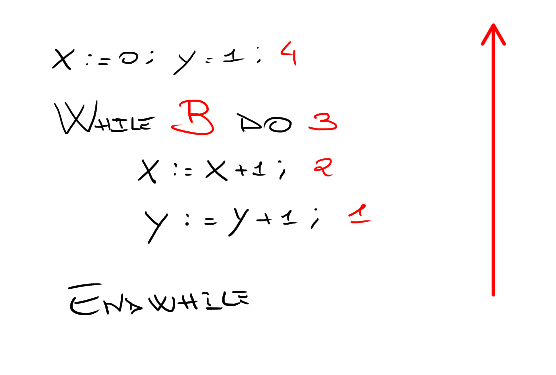
\includegraphics[width=0.7\textwidth]{img/IterationSteps.png}
				      			\end{figure}
				     
				      							      			  
				      			\paragraph{Trovare un'invariante}
				      			Concentriamoci sull'iterazione cercando un'invariante. \textbf{Una strategia
				      			semplice è quella di simulare i primi passi di una esecuzione, prendendo spunto dagli elementi nella post condizione.} Supponiamo che $N$ non sia nullo. Seguendo le due variabili $i$ e $s$ nelle varie
				      			iterazioni (procedendo verso destra nella tabella) e procedendo in modo
				      			\textit{simbolico} per $s$ (usando quindi il simbolo $x$ direttamente):
				      			\begin{table}[H]
				      				\centering
				      				\begin{tabular}[H]{c|ccccc}
				      					i & 0 & 1   & 2     & 3     & $\ldots$ \\
				      					s & 1 & $x$ & $x^2$ & $x^3$ & $\ldots$ 
				      				\end{tabular}
				      			\end{table}
				      			Si noti che $s= x^i$ sembrerebbe la nostra invariante, dimostriamo ciò tramite ricordando che 
				      			\[\{i\land B\}\,\,\, C\,\,\,\{i\}\] rappresenta la premessa della regola d'interazione, che equivale in questo caso a:
				      			\[\{s=x^i\land i<N\}\mbox{ \textit{C} }\{s=x^i\}\]
				      			Procedo quindi con la dimostrazione, utilizzando l'assegnamento proposto dalla \ref{AssignmentRule} avremo:
				      			\[\vdash_{ass}\{sx=x^{i+1}\}\mbox{ \textit{C} }\{s=x^i\}\]
				      			infatti i due assegnamenti sono \emph{indipendenti}, permettendo di applicare
				      			in una sola volta due regole di assegnamento.\\
				      			Sapendo che $s\cancel{x}=x^{i+\cancel{i}}\implies s=x^i$. Abbiamo quindi mostrato
				      			che:
				      			\[\vdash \{s=x^i\}\mbox{ \textit{C} }\{s=x^i\}\]
				      	
				      			Dimostrando che abbiamo effettivamente l'invariante $s= x^i$ (poiché non varia all'inizio e alla fine, e nel dettaglio
				      			abbiamo trovato un \textbf{invariante forte}, che lo è a priori rispetto alla
				      			condizione booleana $B$).\\
				      							      			  
				      			\paragraph{Risoluzione del problema data l'invariante}
				      		`Ricordiamo che l'obbiettivo è quello di derivare $\{s=x^i\land i<N\}$, ma facendo attenzione possiamo notare questa condizione è sicuramente più forte della precedente, ovvero:
				      			\[\{s=x^i\land i<N\} \implies \{s=x^i\}\]
				      			Quindi possiamo riscrivere il tutto come mediate la regola dell'implicazione:
				      		\[\vdash_{impl} \{s=x^i\land i<N\}\mbox{ \textit{C} }\{s=x^i\}\]		
				      			posso quindi applicare la regola dell'iterazione avendo la premessa corretta e
				      			ottenendo quindi:
				      			\[\vdash_{iter}\{s=x^i\}\mbox{ \textit{W} }\{s=x^i\land i\geq N\}\]
				      			ma la post-condizione non ci sta implicando $s=x^N$, per avere:
				      			\[\{N\geq 0\}\mbox{ \textit{P} }\{s\cceq x^N\}\]
				      			bisogna quindi \textbf{rafforzare} l'invariante, in modo che l'invariante
				      			implichi che alla fine dell'esecuzione $i=N$.\\
				      			\paragraph{Rafforzamento dell'invariante}
				      			Procediamo quindi con una nuova ipotesi, cercando di dimostrare che $i\leq N$
				      			è un'invariante:
				      			\[\{i\leq N\land i<N\}\mbox{ \textit{C} }\{i\leq N\}\]
				      			Questa pre-condizione contiene una formula che è più restrittiva dell'altra.
				      			Ricordando che il programma $C$ possiede due assegnamenti: $i := i + 1; s := s * x;$. Avremo:
				      			\[\mbox{ \textit{C} }\{i\leq N\} \implies \vdash_{ass}\{i+1\leq N\}\mbox{ \textit{C} }\{i\leq N\} \]
				      			ma sapendo che $i<N\implies i+1\leq N$ ottengo:
				      			\[\vdash_{impl}\{i< N\}\mbox{ \textit{C} }\{i\leq N\}\]
				      			Dimostrando quindi che è un'invariante.\\
				      			\paragraph{Risoluzione del problema dato il rafforzamento dell'invariante}
				      			Passo quindi all'iterazione:
				      			\[\vdash_{iter}\{i\leq N\}\mbox{ \textit{W} }\{i\leq N\land i\geq N\}\]
				      			e la post-condizione è uguale a dire che $i=N$.\\
				      			Considerando quindi i due invarianti ottengo:
				      			\[\vdash_{iter}\{s=x^i\land i\leq N\}\mbox{ \textit{W} }
				      				\{s=x^i\land i= N\}\]
				      				\paragraph{Dimostrazione per gli assegnamenti iniziali}
				      				Per far si che l'invariante descritto sia effettivamente valido, dobbiamo controllare se esso è valido prima dell'istruzione iterativa.
				      				Dobbiamo quindi dimostrare anche la parte degli assegnamenti iniziali \textbf{"A"}, ovvero $i := 0; s := 1;$:
				      				\begin{align}
				      					\{N\geq 0\}\mbox{ \textit{A} }\{s=x^i\land i\leq N\} 
				      					\label{PrimaParte}                                   
				      				\end{align}
				      				Bisogna infatti vedere se anche le condizioni iniziali permettono
				      				all'invariante doppio di restare tale.\\
				      				applichiamo quindi due volte l'assegnamento (partendo dal fondo); il primo con
				      				$s\cceq 1$: 
				      				\[\vdash_{ass}\{1=x^i\land i\leq N\}\mbox{ $s\cceq 1$ }\{s=x^i\land i\leq N\}\]
				      				Utilizzando la pre-condizione appena descritta come post-condizione, passo quindi a $i\cceq 0$ seguendo il nuovo ordine delle condizioni:
				      				\[\vdash_{ass}\{1=x^0\land 0\leq N\}\mbox{ $i\cceq 0$ }\{1=x^i\land i\leq N\}\]
				      				Ricordando che la regola di derivazione per la \textbf{sequenza} (si veda la \ref{SequenceRule}) equivale a:   \[\frac{\{p\}\,\, C_1\,\,\{q\}\,\,
				      					\,\,\{q\}\,\, C_2\,\,\{r\}}{\{p\}\,\, C_1;C_2\,\,\{r\}}\] \\applichiamo quindi la sequenza con la \ref{PrimaParte} (sapendo $1=x^0$ è sempre vero):
				      				\[\vdash_{seq}\{N\geq 0\}\mbox{ \textit{A} }\{s=x^i\land i\leq N\}\]
				      				completando la dimostrazione.\\
				      				\end{esempio}
				      				\begin{esempio}
				      					Vediamo quindi un esempio completo.\\
				      					Si prenda il seguente programma:
				      					\begin{listing}[H]
				      						\begin{lstlisting}
      quo ~ 0; rem ~ x;
      while rem > y do
        rem ~ rem - y;
        quo ~ quo + 1;
      endwhile  
				      						\end{lstlisting}
				      						\caption{Programma $P$}
				      						\label{E:W}
				      					\end{listing}
				      					Immaginiamo che $x$ e $y$ siano state lette da standard input e che siano quindi reperibili nel programma. Vogliamo dimostrare che:
				      					\[\{x\geq 0 \land y\geq 0\}\mbox{ \textit{P} }\{x=quo*y + rem \land 0 \leq rem \land rem < y\}\]
				      					Quindi il programma dovrebbe calcolare il quoziente e il resto della divisione tra x e y. \\ 
				      					\begin{nota}
				      					$ rem < y := \neg B $, quindi al termine dell'esecuzione questa post-condizione sarà già garantita.
				      					\end{nota}
				      					\paragraph{Passi da seguire}
				      					Ripetiamo ancora una volta i passi da eseguire nel processo:
				      			\begin{enumerate}
				      			    \item Troviamo una possibile invariante
				      			   \item Dimostriamo che sia un'invariante sfruttando la \[\{i\land B\}\,\,\, C\,\,\,\{i\}\]
				      			   sugli assegnamenti interni al ciclo.
				      			   \item Dalla dimostrazione precedente possiamo sfruttare la regola iterativa \ref{IterationRulePartial} per dimostrare che l'invariante è valida anche per $W$.
				      			   \item Dimostriamo che l'invariante è valida anche per gli assegnamenti iniziali prima del ciclo $W$.
				      			\end{enumerate}
				      					\paragraph{Trovare un'invariante}
				      					\begin{nota}
				      					In genere l'invariante viene calcolata partendo dalla post-condizione della regola che vogliamo raggiungere.
				      					\end{nota} 
				      									      					\begin{table}[H]
				      						\centering
				      						\begin{tabular}[H]{c|ccccc}
				      							quo & 0   & 1     & 2      & 3      & $\ldots$ \\
				      							rem & $x$ & $x-y$ & $x-2y$ & $x-3y$ & $\ldots$ 
				      						\end{tabular}
				      					\end{table}

				      					In questo caso notiamo che delle possibili invarianti possono essere:
				      					\begin{itemize}
				      						\item $x=quo*y + rem$
				      						\item $0 \leq rem$
				      					\end{itemize}
				      					Impostiamo la tripla da verificare secondo la formula dell'iterazione parziale ( \ref{IterationRulePartial}):\\
				      					\begin{align}
				      						\{x=quo*y + rem\,\,\,\land\,\,\, 0 \leq rem\,\,\,\land\,\,\, rem\geq y\}\,\,\, C\,\,\,\{i\} 
				      						\label{ToCheck}                                                                          
				      					\end{align}
				      					Sapendo che C riguarda due assegnamenti indipendenti, nello specifico: $        rem := rem - y; quo := quo + 1;$, eseguiamo la regola dell'assegnamento ( \ref{AssignmentRule}) direttamente su entrambe le sostituzioni.
				      					\[\vdash_{ass}\{x=(quo+1)*y + (rem -y)\,\,\,\land\,\,\, 0 \leq (rem-y)\}\,\,\, C\,\,\,\{i\}\]
				      					
				  \begin{nota}
				   $rem \geq y $, non è contenuta nella formula chiaramente perché stiamo costruendo a posteriori (dal basso verso l'alto) la \ref{ToCheck} partendo da: \[\{i\}\,\,\, C\,\,\,\{i\}\]
				   \newline
				  \end{nota}
				      					Svolgendo i calcoli si ottiene la formula che coincide con la \ref{IterationRulePartial} (quindi con $B = rem\geq y$ ):
				      					\[\vdash_{}\{x=quo*y + rem\,\,\,\land\,\,\, rem\geq y\}\,\,\, C\,\,\,\{i\}\]
				      					\begin{nota}
				      					 Sappiamo che $y\geq0$ poiché è una pre-condizione del programma.
				      					\end{nota} 
				      					Sfruttando la regola \ref{IterationRulePartial} allora si ottiene:
				      					\[\vdash_{iter}\{x=quo*y + rem\,\,\,\land\,\,\, rem\geq y\}\,\,\, W\,\,\,\{x=quo*y + rem\,\,\,\land\,\,\, rem\geq 0\,\,\,\land\,\,\, rem<y\}\]
				      					\paragraph{Dimostriamo che vale per gli assegnamenti iniziali}
				      					Dobbiamo dimostrare che le due invarianti hanno valore dopo gli assegnamenti iniziali ($quo := 0; rem := x;$) e che $y\geq0$. 
				      					Dimostriamo allora la regola:
				      					\begin{align}
				      						\{x\geq 0 \land y\geq 0\}\mbox{ \textit{A} }\{x=quo*y + rem\,\,\,\land\,\,\, rem \geq 0\} 
				      						\label{ToCheck2}                                                                         
				      					\end{align}
				      					\[\vdash_{ass}\{x=x\,\,\,\land\,\,\, rem \geq 0\}\mbox{ \textit{A} }\{x=quo*y + rem\,\,\,\land\,\,\, rem \geq 0\}\]
				      					\[\vdash_{}\{x \geq 0\}\mbox{ \textit{A} }\{x=quo*y + rem\,\,\,\land\,\,\, rem \geq 0\}\]
				      				\end{esempio}
				      				\subsubsection{Correttezza totale}
				      				Analizziamo ora il caso in cui non si abbia certezza di terminazione di
				      				un'iterazione:
				      				\[\{p\}\mbox{ while \textit{B} do \textit{C} endwhile }\{q\}\]
				      								      				\begin{definizione}
				      					Se si esegue $W$  a partire da uno stato in cui varrà $p$ e dimostriamo che l'esecuzione termina allora nello stato finale vale $q$.
				      				\end{definizione} \vspace{5mm} %5mm vertical sspace

				      				Distinguiamo i due tipi di correttezza, dal punto di vista della derivabilità,
				      				tramite: 
				      				\[\vdash^{parz}\{p\}\mbox{ C }\{q\}\]
				      				\[e\]
				      				\[\vdash^{tot}\{p\}\mbox{ C }\{q\}\]
				      				Dal punto di vista semantico non ha invece senso distinguere di due casi e
				      				quindi si ha solo:
				      				\[\vDash\{p\}\mbox{ C }\{q\}\]
				      				In quanto dal punto di vista semantico o si ha terminazione o non si ha, non si
				      				hanno casistiche differenti a seconda di correttezza totale o parziale.\\
				      				Bisognerà quindi dimostrare la terminazione.\\
				      				Studiamo il caso semplice dove:
				      				\[W=\mbox{ while \textit{B} do \textit{C} endwhile }\]
				      				Cerchiamo un'espressione \textbf{aritmetica} $E$ che chiameremo \textbf{variante}, dove compaiono le variabili del
				      				programma, costanti numeriche e operazioni aritmetiche. Cerchiamo anche un
				      				\textbf{invariante di ciclo} $i$ (che quindi è una formula) per $W$. $E$ e $i$
				      				devono soddisfare due condizioni:
				      				\begin{enumerate}
				      					\item $i\implies E\geq 0$, quindi se vale $i$ allora l'espressione aritmetica
				      					      ha valore $\geq 0$ (il valore di $E$ lo ottengo eseguendo le operazioni sulle
				      					      costanti e sui valori, in quello stato della memoria, delle variabili)
				      					      \label{ConditionTotalCorrectness1}
				      					\item $\vdash^{tot}\{i\land B\land E=k\}\mbox{ C }\{i\land E<k\}$.
				      					\begin{itemize}
				      					    \item Dove
				      					      nella pre-condizione (che quindi supponiamo sia valida) abbiamo la congiunzione logica tra l'invariante $i$, la
				      					      condizione di ciclo $B$ e tra $E=k$, avendo prima assegnato a $k$ il valore
				      					      effettivo di $E$ nello stato in cui iniziamo a computare $C$. Il valore $k$ quindi non
				      					      deve essere una variabile del programma e non deve apparire in $C$
				      					      (rappresentante il corpo della singola iterazione). Se vale la
				      					      condizione 1 e l'invariante sappiamo che $E\geq 0\implies k\geq 0$. 
				      					      \item La
				      					      post-condizione è formata dall'invariante $i$ e dal fatto che il valore di $E$
				      					      dopo l'esecuzione sia strettamente minore di $k$ (che è il valore di $E$ prima
				      					      dell'esecuzione). \textbf{In pratica $E$ decresce ad ogni singola iterazione, ovvero
				      					      	ad ogni esecuzione di $C$.}\\
				      					      La notazione $\vdash^{tot}$ serve a escludere che $C$ abbia altri cicli
				      					      annidati, portando a dover dimostrare che anche i cicli interni
				      					      terminano pochè $E$ è destinata a decrementarsi un numero \textbf{finito} di volte (essendo limitata da $k$ ad essere maggiore o uguale a zero) . Per praticità quindi supponiamo di non avere cicli interni (stiamo
				      					      partendo dal ciclo più interno)
				      					\end{itemize}
				      		
				      					      \label{ConditionTotalCorrectness2}
				      				\end{enumerate}
				      				In pratica, nella seconda condizione, uso $E$ per concludere che una singola
				      				esecuzione dell'iterazione ci porta in uno stato in cui vale l'invariante, dove
				      				può valere o meno $B$ (che potrebbe portare all'uscita dall'iterazione) ma in
				      				cui $E$ ha un valore diverso, minore a quello di partenza ma mai minore di zero per
				      				la prima condizione (in quanto l'invariante è sempre valido e per la prima condizione ciò implica che $E \geq 0$). Quindi, a un
				      				certo punto, $E$ raggiungerà il valore minimo e in quel momento o $B$ sarà falsa oppure
				      				si avrà una contraddizione ($E$ dovrebbe diventare negativo), quindi si ha la
				      				terminazione. \\
				      				\textbf{Quindi se e solo se abbiamo dimostrato le due condizioni possiamo affermare che}:
				      				\[\vdash^{tot}\{i\}\mbox{ W }\{i\land\neg B\}\]
				      				è anche la conclusione della regola di derivazione dell'iterazione in caso
				      				di correttezza \textbf{totale} (Per maggiori informazioni ricontrollare la \ref{IterationRulePartial}).\\
				      				Possiamo anche osservare due cose:
				      				\begin{enumerate}
				      					\item $E$ non è una formula logica ma un'espressione aritmetica con valore
				      					      numerico ($E\geq 0$ è una formula logica)
				      					\item qualora si abbia $E=0$ non si hanno problemi, $0$ è solo un esempio,
				      					      potremmo riscrivere la prima condizione come $E\geq n$, con $n$ qualsiasi
				      					      numero intero, basta che sia ben definito per poter permettere la ripetizione
				      					      finita delle iterazioni
				      				\end{enumerate}
				      				\begin{nota}
				      				L'invariante della correttezza totale non è sempre quello di quella
				      				parziale, magari è uguale, magari diverso o anche uguale solo in parte.
				      				\end{nota}
				      			    
				      				\paragraph{Rintracciamento dell'espressione aritmetica variante E}
				      				Spesso si è visto che $E$ si ricava da $B$. Se $B$ è della forma $x>y$ 
				      					allora $E$ sarà $x-y$. In caso di $<$, $\leq$ e $\geq$ allora bisognerebbe ricondursi a $>$.
				      				\begin{esempio}
				      					Vediamo un esempio chiarificatore.\\
				      					Dato il programma (una sorta di conto alla rovescia):
				      					\begin{listing}[H]
				      						\begin{lstlisting}
      while x > 5 do
        x ~ x - 1;
      endwhile  
				      						\end{lstlisting}
				      						\caption{Programma $P$}
				      						\label{E:t}
				      					\end{listing}
				      					studio la correttezza totale della tripla:
				      					\[\{x>5\}\mbox{ P }\{x=5\}\]
				      					\paragraph{Ricerca variante e Invariante}
				      					Innanzitutto Cerchiamo un variante $E$, che decresce a ogni singola iterazione, e
				      					un'invariante $i$ come descritti sopra. Quindi, secondo la regola  \ref{ConditionTotalCorrectness1}, qualora ci sia
				      					l'invariante $i$ allora  $E\geq 0$.\\
				      					In merito ad $E$ notiamo che nel corpo dell'iterazione abbiamo un solo	comando, dove il valore della variabile $x$ viene decrementato, quindi, facendo i calcoli su $B$, potremmo pensare di prendere in considerazione 
				      					\[E: x - 5\]
				      					Dovendo però garantire che $E\geq 0$ in relazione a un dato invariante $i$, allora scegliamo:
				      					\[i: x \geq 5\] \\		
				      					\begin{nota}
				      					Non sempre posso ottenere una corrispondenza tra variante e
				      						invariante.
				      					\end{nota}
				      					Presi questo invariante e questo variante verifichiamo le regole \ref{ConditionTotalCorrectness1} e \ref{ConditionTotalCorrectness2}:
				      					\begin{enumerate}
				      						\item $x\geq 5\implies x-5\geq 0$ è ovviamente corretto perché si ottiene
				      						      che $x\geq 5\implies x \geq 5$ (infatti questo è il motivo per cui si è
				      						      scelto $x-5$ come variante)
				      						\item $\vdash^{tot}\{x\geq 5\land x>5\land x-5=k\}\,\,\, x\cceq
				      						      x-1\,\,\,\{x\geq 5\land x-5<k\}$\\
				      						      applichiamo quindi la regola dell'assegnamento (\ref{AssignmentRule}) (che si applica anche per la
				      						      correttezza totale) e ottengo la pre-condizione per la post-condizione
				      						      $\{x\geq 5\land x-5<k\}$:
				      						      \[\{x-1\geq 5\land x-1-5<k\}=\{x\geq 6\land x-6 < k\}\]
				      						      che però è diversa da $\{x\geq 5\land x>5\land x-5=k\}$.\\
				      						      Cerchiamo quindi di applicare la regola dell'implicazione. Riguardando la
				      						      pre-condizione originale noto che $x>5$ è ``più fortè' di $x\geq 5$ e quindi
				      						      quest'ultimo può essere trascurato. Ricordando che stiamo lavorando su
				      						      valori interi si ha che $x>5\implies x\geq 6$. Inoltre, sempre per il fatto
				      						      che lavoriamo su numeri interi, \\
				      						      $x-5=k\implies x-6<k$ e quindi:
				      						      \[\{x\geq 5\land x>5\land x-5=k\}\implies \{x\geq 6\land x-6 < k\}\]
				      					\end{enumerate}
				      					Abbiamo quindi dimostrato che il programma termina e vale la tripla
				      					iniziale.\\
				      					Qualora avessimo dovuto dimostrare la correttezza parziale si sarebbe dovuto
				      					procedere riutilizzando lo stesso invariante e procedendo studiando la
				      					negazione di $B$, ovvero $x\leq 5$ (che insieme danno la post-condizione).
				      				\end{esempio}
				      				\begin{esempio}
				      					vediamo un esempio dove non si ha alcuna variabile che decrementa nel corpo
				      					dell'iterazione:
				      					\begin{listing}[H]
				      						\begin{lstlisting}
      while x < 5 do
        x ~ x + 1;
      endwhile  
				      						\end{lstlisting}
				      						\caption{Programma $P$}
				      						\label{E:ti}
				      					\end{listing}
				      					studio la correttezza totale della tripla:
				      					\[\{x<5\}\mbox{ P }\{x=5\}\]
				      					Dal punto di vista della correttezza parziale ragioniamo come al solito mentre
				      					per la correttezza totale la situazione è un po' diversa.\\
				      					Ovviamente non posso usare $x$ come variante ma posso sicuramente usare, per
				      					esempio, $-x$, che sicuramente decresce visto che $x$ cresce, in entrambi i
				      					casi a ogni iterazione. Riprendendo l'esempio sopra quindi posso usare $x\leq
				      					5$ come invariante e, al posto di $-x$ (che comunque andrebbe bene), secondo un
				      					ragionamento simile allo scorso esempio, $5-x$ come variante (si noti che
				      					anche questo $E$ è ricavabile da $i$, anche se questo non è sempre attuabile).
				      					Il resto della dimostrazione è analoga all'esempio precedente.
				      				\end{esempio}
				      				\subsection{Esempi di Ricapitolazione}
				      				\begin{esempio}
				      					\begin{lstlisting}
	
	   p ~ 1 ; y ~ b; 
      while y > 0 do
        p ~ p * x;
        y ~ y - 1;
      endwhile      						\end{lstlisting}
				      vogliamo sapere se vale la regola:
				      
				      \[\{b \geq 0\}P\{p = x^b\}\] 
				      
				      \paragraph{Correttezza Parziale: Trovare un'invariante}
				      Consideriamo inizialmente la correttezza parziale.
				     
				      \[inv: p = x^{b-y} \land y \geq 0\]
				      \paragraph{Dimostro che inv è un'invariante di ciclo per W}
				      
				      \[inv: p = x^{b-y} \land y \geq 0\]
				      dobbiamo quindi dimostrare che:
				      \[\{x^{b-y} \land y \geq 0 \land y > 0\}C\{x^{b-y} \land y \geq 0\}\] 
				      Si noti dal programma che gli assegnamenti sono indipendenti, quindi applichiamo la \ref{AssignmentRule} simultaneamente a entrambe:
				      \[C\{x^{b-y} \land y \geq 0\}\] 
				      Semplificando viene dimostrata la formula. Si noti che per la regola dell'implicazione $y > 0 \implies y \geq 0$.
				      \[\vdash^{}\{x^{b-y} \land y > 0 \}C\{x^{b-y} \land y \geq 0\}\]
				      Quindi abbiamo dedotto la premessa per eseguire la regola d'iterazione per la correttezza parziale. \ref{IterationRulePartial}.
				      \paragraph{Applichiamo la regola dell'iterazione}
            
  				      \[\vdash^{iter}\{x^{b-y} \land y \geq 0 \}W\{x^{b-y} \land y \geq 0\ \land y \leq 0\}\]
  				       
				      Si noti che $ y \geq 0\ \land y \leq 0 \implies y = 0$. Allora giungiamo alla conclusione:
				       				        \begin{align}
  				       \vdash^{}\{x^{b-y} \land y \geq 0 \}W\{x^b\}
      				        \label{Example1}
 				        \end{align}

				      \paragraph{Controlliamo l'invariante dopo l'assegnamento iniziale}
                        Controlliamo se vale la regola:
                         \[\{b \geq 0\}A\{x^{b-y} \land y \geq 0\}\]
                         
                         Utilizzo sempre la \ref{AssignmentRule} in maniera indipendente:
                        
                        \[A\{x^{b-y} \land y \geq 0\}\]
 				        \[\vdash^{as}\{ True \land b \geq 0 \} A \{ x^{b-y} \land y \geq 0\}\]
 				        \begin{align}
      				        \vdash^{imp}\{b \geq 0 \}A\{x^{b-y} \land y \geq 0\}
      				        \label{Example2}
 				        \end{align}
				      \begin{nota}
				      Applicando la regola della sequenza tra \ref{Example1} e \ref{Example2} si giunge alla conclusione.
				      \end{nota} 
                    \paragraph{Correttezza Totale: Invariante e Variante}
                    Scegliamo:
                    \[E: y\]
			      Dovendo però garantire che $E\geq 0$ in relazione a un dato invariante $i$, allora Scegliamo
			      \[i: y \geq 0\] 
			      Cerchiamo di verificare secondo la regola \ref{ConditionTotalCorrectness2} della correttezza totale:
			      \[\vdash^{tot}\{y \geq 0 \land y > 0 \land y=k\}\mbox{ y := y - 1 }\{y \geq 0\land y<k\}\]
			      
			      \[\mbox{ y := y - 1 }\{y \geq 0\land y < k\}\]

			      \[\vdash^{as}\{y - 1 \geq 0\land y-1 < k\}\mbox{ y := y - 1 }\{y \geq 0\land y<k\}\]
			      
			      \[\vdash^{imp}\{y > 0 \land y-1 < k\}\mbox{ y := y - 1 }\{y \geq 0\land y<k\}\]
			      
			      \begin{nota}
			      $y = k \implies y - 1 < k$
			      \end{nota}
			      
				    \end{esempio}   
				     
				     
				     \subsection{Correttezza e Completezza}
				      				In generale quando si sviluppa una logica, con un apparato deduttivo e
				      				un'interpretazione delle formule, siamo interessati a due proprietà generali
				      				della logica e dell'apparato deduttivo:
				      				\begin{enumerate}
				      					\item \textbf{correttezza}, ovvero il fatto che tutto quello che si può
				      					      derivare con l'apparato deduttivo è effettivamente vero, ovvero
				      					      $'\vdash' \implies '\vDash'$. Quindi se una tripla è derivabile è anche vera
				      					\item \textbf{completezza}, ovvero il fatto che l'apparato deduttivo sia in
				      					      grado di derivare tutte le formule vere (ovvero tutte le triple). Si ha
				      					      quindi $'\vDash' \implies '\vdash'$
				      				\end{enumerate}
				      				Per la logica di Hoare vale la correttezza ma vale una proprietà di completezza \textit{relativa} in quanto nel corso di una dimostrazione di completezza
				      				occorre a volte usare deduzioni della logica proposizionale ma tali formule
				      				parlano anche di operazioni aritmetiche. Si ha che l'aritmetica può essere
				      				formalizzata attraverso un linguaggio logico con degli assiomi e delle regole di
				      				inferenza. Si hanno però i \textbf{teoremi d'incompletezza dell'aritmetica} di
				      				G\"{o}del che dicono che l'aritmetica come teoria matematica è incompleta in
				      				quanto ci sono formule scritte nel linguaggio dell'aritmetica che sono vere ma
				      				non sono dimostrabili. Questa incompletezza si riverbera sulla logica di Hoare,
				      				che comunque, dal punto di vista deduttivo sulle triple, è completa.
				      				\subsection{Pre-condizione debole: ricerca della migliore precondizione}
				      				Dato un comando $C$ e una post-condizione $q$ di
				      				$C$. Si cerca $p$ tale per cui:
				      				\[\vDash\{p\}\mbox{ C } \{q\}\]
				      				Sia valida e quindi vera.\\
				      				\begin{esempio}
				      					Suppongo di avere come comando un singolo assegnamento $y\cceq 2\cdot x-1$ e
				      					come post-condizione $\{y>x\}$.\\
				      					Cerchiamo possibili precondizioni che, dopo l'assegnamento, portino a quella
				      					post-condizione. Ovviamente si avrebbero infiniti valori di $x$ che consentono
				      					di arrivare alla post-condizione (nonché altrettanti che non lo permettono). 
				      				\end{esempio}
				      				L'obiettivo riguarda la ricerca della migliore pre-condizione per arrivare ad una data
				      				post-condizione, ma per far ciò serve un \textbf{criterio di confronto}. Introduciamo quindi alcuni simboli e nozioni utili:
				      				\begin{itemize}
				      					\item $V$ è l'insieme delle variabili di $C$
				      					\item $\Sigma=\{\sigma|\,\sigma:V\to\mathbb{Z}\}$ è l'insieme degli stati
				      					      della memoria (ricordando che posso avere solo valori interi nel nostro
				      					      linguaggio)
				      					\item $\Pi$ è l'insieme di tutte le formule sull'insieme $V$
				      					\item $\sigma \vDash p$ significa che la formula $p$ è vera nello stato
				      					      $\sigma$ e si ha che $\vDash\subseteq\Sigma\times \Pi$, con $\vDash$ che
				      					      indica la veridicità di una formula in uno stato
				      					\item $t(\sigma)=\{p\in \Pi|\,\sigma\vDash p\}$ come la funzione che assegna
				      					      ad uno stato $\sigma$ tutte le formule che sono
				      					      vere in esso.
				      					\item $m(p)=\{\sigma\in \Sigma|\,\sigma\vDash p\}$ come la funzione che
				      					      associa ad una formula $p$ l'insieme di tutti gli stati che soddisfano la formula stessa.
				      				\end{itemize}
				      				\subsubsection{Dualità}
				      				Tra le due funzioni finali si ha una sorta di ``dualità'' e agiscono in modo
				      				speculare tra loro.
				      				\begin{definizione}
				      				     Se, partendo da $\sigma \in \Sigma$ applicassimo $t(\sigma)$ tale per cui risultasse una formula $p \in t(\sigma)$ allora sicuramente $ \sigma \in m(p)$ (fig. \ref{fig:SigmaAndPi}).
				      				     \[p \in t(\sigma) \iff \sigma \in m(p) \,\,\,\,\,\, \forall p, \sigma \]
				      				\end{definizione}
				      				\begin{figure}[H]
                                        \centering 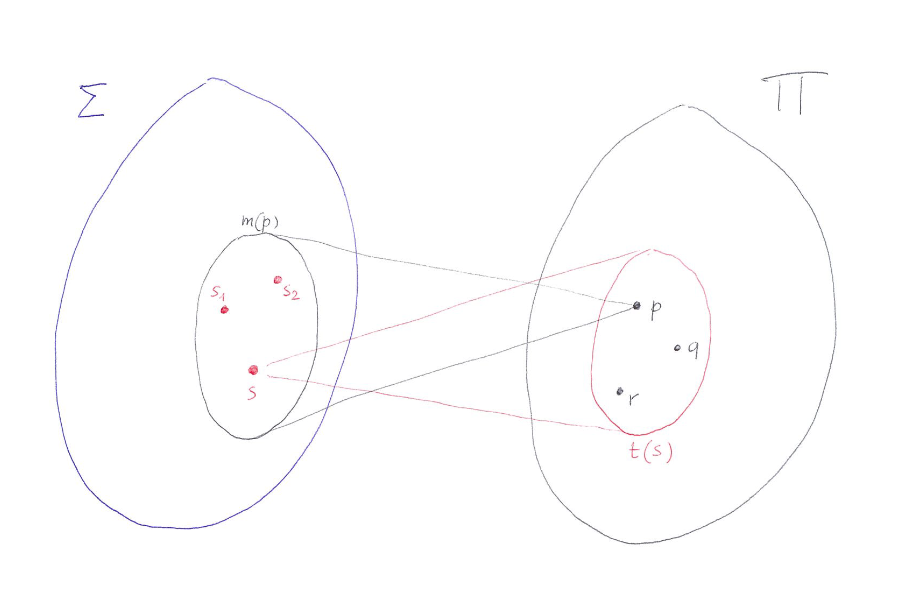
\includegraphics[width=1\textwidth]{img/VENN.png}
                                        \caption{Correlazione tra $\Sigma$ e $\Pi$.}
                                        \label{fig:SigmaAndPi}
                                    \end{figure}
				      				Si possono fare altre osservazioni su queste due funzioni. \\
				      				Prendiamo due formule $p$ e $q$ e cerchiamo di capire se è possibile avere
				      				$m(p)=m(q)$, ovvero cerchiamo di capire se l'insieme degli stati in cui vale $p$ è uguale a quello di $q$. La risposta alla domanda viene data grazie al concetto di \textbf{equivalenza
				      					tra formule}: difatti due formule possono essere vere negli stessi stati. \\ 
				      					Fissati due stati $\sigma_1$ e $\sigma_2$ chiediamoci ora se possano
				      				appartenere allo stesso insieme di formule. In questo caso la risposta è
				      				negativa, in quanto se i due stati sono distinti allora ci deve essere almeno
				      				una variabile $x$ che ha valore diverso nei due stati.\\
				      				\subsubsection{Sottoinsiemi}
				      			\begin{definizione}
				      			    	Dato $S\subseteq \Sigma$, sottoinsieme di stati, e $F\subseteq\Pi$, sottoinsieme di formule, si
				      				ha che:
				      				\begin{itemize}
				      					\item $t(S)=\{p\in \Pi|\,\forall\,\sigma\in S,\,\,\,\sigma\vDash
				      					      p\}=\bigcap_{\sigma\in S}t(\sigma)$ (ragioniamo quindi su tutti gli stati di $S$
				      					      e quindi sulle formule che sono vere in tutti questi stati) 
				      					\item $m(F)=\{\sigma\in \Sigma|\,\forall\, p\in F\,\,\,\sigma\vDash
				      					      p\}=\bigcap_{p\in \Pi}m(p)$ (ragioniamo quindi su tutte le formule di $\Pi$
				      					      e quindi su tutti gli stati in devono essere soddisfatte tutte queste formule) 
				      				\end{itemize}
				      				\begin{corollario}
				      				            $S\subseteq m(t(S))$ e $F\subseteq
				      				t(m(F))$
				      				\end{corollario}
				      				\begin{corollario}
				      				             Dati $A\subseteq B$, si può dimostrare che $m(B)\subseteq
				      				m(A)$
				      				\end{corollario}
				      			\end{definizione}
				      			 \subsubsection{Relazione tra logica proposizionale e stati}
				      				Si ha un rapporto tra la logica proposizionale (coi suoi connettivi logici) e
				      				l'insieme di stati ($p$ e $q$ sono formule di $\Pi$): 
				      				\begin{itemize}
				      					\item $m(\neg p)=\Sigma \,\,\backslash \,\, m(p)$, quindi il complemento
				      					      insiemistico di $p$
				      					\item $m(p\lor q)=m(p)\cup m(q)$, quindi all'unione dei due insiemi  
				      				
				      				\end{itemize}
				      				L'implicazione merita un discorso a parte in quanto ha si può vedere sotto due punti di vista:
				      				\begin{itemize}
				      					\item come \textbf{operatore logico}, che comporta che $p\implies q= \neg p\lor q$
				      					      e in tal caso si ha, in linea a quanto detto per gli altri connettivi:
				      					      \[m(p\implies q)= m(\neg p)\cup m(q)\]
				      					\item come \textbf{relazione tra formule}: che si può vedere in modo insiemistico dove se $p$ implica $q$ (in tutti in
				      					      casi in cui è vera $p$ è vera $q$) allora
				      					      $m(p)\subseteq m(q)$, intendendo che $q$ è ``\textbf{più debolè}' di $p$. Ovvero viene vista come una formula che
				      					      ci dà una conoscenza inferiore/incertezza maggiore essendo $q$ corrispondente a un insieme più
				      					      grande di stati. 
				      				\end{itemize}
				      				Posso quindi capire come definire la pre-condizione migliore per ottenere una
				      				tripla valida, insieme al comando $C$ e alla post-condizione.\\
				      				\subsubsection{Criterio di scelta della pre-condizione migliore}
				      			    \begin{definizione}
				      			        Un modo per specificare la pre-condizione migliore per ottenere una
				      				tripla valida è quello di definire la più
				      				debole pre-condizione $p$ che forma una tripla valida:
				      				\[\vDash \{p\}\mbox{ C }\{q\}\] \\
				      				Se $p$ è la pre-condizione più debole allora corrisponde al più grande insieme di
				      				stati tale per cui la tripla è valida, ovvero il più grande insieme di stati a partire dai quali l'esecuzione di $C$ porta ad uno stato in $m(q)$.
				      			    \end{definizione} \vspace{5mm} %5mm vertical space
				      				Questa è una scelta ragionevole perché è la pre-condizione che impone meno
				      				vincoli sullo stato iniziale, infatti determina tutti gli stati iniziali che
				      				garantiscono il raggiungimento della post-condizione. È sempre possibile
				      				calcolare la pre-condizione più debole.\\
				      				\begin{nota}
				      				Se trovassimo come pre-condizione più debole l'insieme vuoto di formule allora sicuramente non saremo mai in grado di arrivare alla post-condizione.
				      				
				      				\begin{esempio}
				      				    Immaginiamo il programma:
				      				    \[\mbox{ x:=5 }\{x < 0\}\]
				      				    
				      				    allora sicuramente la pre-condizione sarebbe l'insieme vuoto, ovvero la costante $F$. Per cui non saremo mai in grado di arrivare alla post-condizione.
				      				\end{esempio}
				      				\end{nota}
				      				\begin{definizione}
				      				    La pre-condizione più debole viene implicata da tutte le altre che soddisfano la tripla comune.
				      				\end{definizione}
				      			\begin{definizione}
				      			    	Indichiamo, fissati $C$ comando e $q$ formula di post-condizione, con $wp(C, q)$
				      				la pre-condizione più debole (\textbf{weakest precondition (\textit{wp})}).
				      			\end{definizione}
				      				\begin{definizione}[proprietà fondamentale della condizione più debole]
				      					  $\vDash\{p\}\mbox{ C }\{q\}$ (quindi la tripla è vera) sse:
				      					\[p\implies wp(C, q)\]
				      					Ovvero la tripla è vera sse tutte le pre-condizioni implicano quella più debole, ovvero ogni pre-condizione è piu \textbf{forte}.
				      					\begin{nota}
				      					Si ricorda che la pre-condizione più debole per definizione è la più generale, quindi include tutte le altre.
				      					\end{nota}
				      				\end{definizione}
				      				\begin{definizione}
				      					L'\textbf{esistenza} della pre-condizione più debole è garantita.\\
				      					È garantita inoltre l'\textbf{unicità} della pre-condizione più debole (a meno
				      					di eventuali equivalenze logiche).
				      				\end{definizione}
				      				\subsubsection{Calcolo della pre-condizione più debole}
				      				Abbiamo visto che la pre-condizione più debole esiste, ma come si fa a calcolarla?
				      				Vediamo quindi la \textit{regola di calcolo}.\\
				      				Si hanno diversi casi a seconda dei tipi di comando:
				      				\begin{itemize}
				      					\item \textbf{assegnamento:} in questo caso la pre-condizione più debole è
				      					      quella determinata dalla regola di derivazione introdotta per la correttezza
				      					      parziale. Quindi dato un assegnamento del tipo $x\cceq E$ e una post-condizione
				      					      $q$ abbiamo che la pre-condizione più debole si ottiene sostituendo in $q$ ogni
				      					      occorrenza di $x$ con l'espressione $E$, ottenendo quindi:
				      					      \[\{q[E/x]\}\]
				      					\item \textbf{sequenza:} in questo caso, se abbiamo la sequenza di due comandi
				      					      $C_1$ e $C_2$ allora la pre-condizione più debole si calcola nel seguente modo:
				      					      calcoliamo la pre-condizione più debole per $C_2$, ottenendo $wp(C_2, q)$, che sarà
				      					      quindi la formula usata come post-condizione per calcolare la pre-condizione più
				      					      debole di $C_1$, ovvero: $wp(C_1, wp(C_2, q))$. Questo non è altro che la
				      					      condizione più debole della sequenza:
				      					      \[wp((C_1;C_2), q)\equiv wp(C_1, wp(C_2, q))\]
				      					\item \textbf{scelta:} in questo caso, avendo:
				      					      \[S=\mbox{ if \textit{B} then \textit{C} else \textit{D} endif }\]
				      					      fisso la post-condizione $q$ e procedo come per la regola di
				      					      derivazione. Separiamo i due casi in cui sia vera $B$ o meno:
				      					      \begin{itemize}
				      					          \item   Se $B$ è vera dobbiamo
				      					      eseguire $C$ quindi calcolo, eseguendo $C$, la pre-condizione più debole
				      					      $wp(C, q)$. 
				      					      
				      					      \item Qualora $B$ non sia vera calcolo, eseguendo $D$, la pre-condizione
				      					      più debole $wp(D, q)$.
				      					      \end{itemize}
				      					       Nel complesso quindi, facendo la disgiunzione dei due
				      					      casi, ottengo: 
				      					      \[wp(S, q)\equiv(B\land wp(C, q))\lor (\neg B\land wp(D, q))\]
				      					    
				      					\item \textbf{iterazione:} 
				      					      \[W=\mbox{while \textit{B} do \textit{C} endwhile}\]
				      					      
				      					      \begin{itemize}
				      					          \item se $\neg B$ è nello stato iniziale dell'iterazione allora il corpo
				      					      non viene eseguito (arrivando direttamente alla post-condizione)
				      					      
				      					      \item invece se
				      					      vale $B$ si può pensare all'iterazione in modo ricorsivo seguendo la regola della sequenza: $C;W$. In modo tale che una volta eseguito $C$ il programma riproporrà nuovamente $W$. Per fissare il concetto basti pensare \textbf{idealmente} (seppur in modo sintatticamente errato) all'eguaglianza $W=C;W$. Questo può accadere in 
				      					      quanto sicuramente almeno una volta si esegue $C$ e lo stesso processo viene riprodotto fin quando $B$ non diventa falso. 
				      					      \end{itemize}   
				      					      Si
				      					      arriva di fatto ad una regola ricorsiva:
				      					      \[wp(W, q)\equiv(\neg B\land q)\lor(B\land wp((C;W), q))\]
				      					      applichiamo quindi la regola della sequenza per la condizione più debole,
				      					      arrivando a:
				      					      \[wp(W, q)\equiv(\neg B\land q)\lor(B\land wp(C, wp(W, q)))\]
				      					      Si nota che questa definizione ricorsiva ha un problema grave: non si ha un
				      					      \textbf{caso base} che risolva la catena di chiamate ricorsive.\\
				      					      Purtroppo non si può usare il ``trucco'' dell'invariante come nella regola di
				      					      definizione e questo comporta che non si ha un vero e proprio algoritmo unico
				      					      ed effettivo per questa regola di ricerca della pre-condizione più debole
				      				\end{itemize}
				      				Si hanno dei casi estremi, ad esempio:
				      				\begin{itemize}
				      					\item precondizioni più deboli sempre false, ad esempio:
				      					      \[wp(x\cceq5, x<0)\equiv\bot\]
				      					      ovvero se assegno a $x$ il valore 5 non avrò mai $x$ negativo,
				      					      ovvero abbiamo un insieme vuoto $\emptyset$ di stati che garantiscono quanto detto
				      					\item precondizioni più deboli sempre vere, ad esempio
				      					      \[wp(x\cceq 5, x\geq0)\equiv\top\]
				      					      ovvero se assegno a $x$ il valore 5 si avrà che $x$ è sempre
				      					      positivo, quindi è vero per qualunque stato iniziale
				      				\end{itemize}
				      				\subsubsection{Esempi vari}
				      				\begin{esempio}
				      					Vediamo un primo esempio semplice con solo la sequenza di due assegnamenti:
				      					\begin{listing}[H]
				      						\begin{lstlisting}
      x ~ x+1;
      y ~ y*x;
				      					\end{lstlisting}
				      					\caption{Programma $P$}
				      					\end{listing}
				      					Dove i due assegnamenti sono rispettivamente $A$ e $B$ e si vuole la
				      					post-condizione $q=x<y$. Cerchiamo quindi $wp(P, q)$.\\
				      					Procediamo con la formula della sequenza (che ricordiamo procede ``a
				      					ritroso'').
				      					\begin{itemize}
				      						\item Parto dal secondo assegnamento, $B$, e calcolo $wp(B, q)$.\\
				      						      Procedo con la regola e applichiamo la sostituzione, ottenendo:
				      						      \[r=wp(B, q)=x<y\cdot x\]
				      						      quindi se $x<y\cdot x$ vale prima dell'esecuzione di $B$ allora sicuramente
				      						      si raggiunge uno stato finale dove vale la post-condizione $q$ 
				      						\item lo stato in cui eseguiamo $B$, che abbiamo sopra chiamato $r$, è
				      						      quello prodotto dall'esecuzione di $A$. Dobbiamo quindi calcolare
				      						      $wp(A, r)$.\\
				      						      Procedo quindi ancora con l'assegnamento, ottenendo:
				      						      \[wp(A, r)\equiv x+1<y(x+1)\]
				      						      che quindi, per composizione, è anche la pre-condizione più debole per $P$ e
				      						      $q$. Bisogna però fare dei controlli.\\
				      						      Uso quindi le regole delle disequazioni:
				      						      \begin{itemize}
				      						      	\item caso 1: $x+1>0\implies y>1$
				      						      	\item caso 2: $x+1=0\implies 0<0$ e quindi non vale $q$
				      						      	\item caso 3: $x+1<0\implies y<0$
				      						      \end{itemize}
				      						      Costruisco quindi la pre-condizione più debole prendendo la disgiunzione
				      						      logica dei due casi validi:
				      						      \[wp(P, q)\equiv(x\geq 0\land y>1)\lor (x<-1\land y<1)\]
				      						      (sempre ricordando che lavoriamo con interi)
				      					\end{itemize}
				      				\end{esempio}
				      				\begin{esempio}
				      					Vediamo un altro esempio:
				      					\begin{listing}[H]
				      						\begin{lstlisting}
      x ~ x+a;
      y ~ y-1;
				      						\end{lstlisting}
				      						\caption{Programma $P$}
				      					\end{listing}
				      					Dove i due assegnamenti sono rispettivamente $A$ e $B$ e si vuole la
				      					post-condizione $q=(x=(b-y)\cdot a)$. Cerchiamo quindi $wp(P, q)$.\\
				      					Nella post-condizione abbiamo una variabile $b$ esterna alla sequenza di interesse
				      					fissato a priori.\\
				      					Come prima ottengo:
				      					\[r=wp(B, q)\equiv(x=(b-y+1)\cdot a)=(x=(b-y)\cdot a)\]
				      					e quindi:
				      					\[wp(A, r)\equiv(x+a=(b-y)\cdot a+a)\]
				      					quindi $x=(b-y)\cdot a$ è un'invariante ed è anche la post-condizione, Quindi $q$
				      					è un'invariante, accezione più forte del termine, per $P$.
				      				\end{esempio}
				      				\begin{esempio}
				      					Vediamo un altro esempio:
				      					\begin{listing}[H]
				      						\begin{lstlisting}
      if y = 0 then
        x ~ 0;
      else
        x ~ x * y;
      endif
				      						\end{lstlisting}
				      						\caption{Programma $P$}
				      					\end{listing}
				      					Dove i due comandi sono rispettivamente $C$ e $D$ e la condizione booleana è
				      					$B$. Come post-condizione vogliamo $q=(x=y)$.\\
				      					Per il caso della scelta bisogna calcolare i due casi e usare poi la
				      					disgiunzione tra essi.\\
				      					Calcolo quindi:
				      					\begin{enumerate}
				      						\item il caso in cui vale $B$: $wp(C, q)=(0=y)$, usando l'assegnamento
				      						\item il caso in cui vale $\neg B$: $wp(D, q)=(x\cdot y)=y$, usando
				      						      assegnamento. La formula però comporta che abbiamo due casi possibili: $y=0\lor
				      						      x=1$ (il secondo appunto se abbiamo $y\neq 0$)
				      					\end{enumerate}
				      					applichiamo quindi la regola della scelta, ottenendo:
				      					\[wp(P, q)\equiv (y=0\land y=0)\lor(y\neq 0\land (y=0\lor x=1))\]
				      					Semplificando si ha che:
				      					\[wp(P, q)\equiv(y=0)\lor(x=1\land y\neq 0)\]
				      				\end{esempio}
				      				\begin{esempio}
				      					Vediamo un altro esempio:
				      					\begin{listing}[H]
				      						\begin{lstlisting}
      while x > 0 do
        x ~ x - 1
      endwhile
				      						\end{lstlisting}
				      						\caption{Programma $P$}
				      					\end{listing}
				      					Con la condizione $B$ e il comando $C$, nel corpo dell'iterazione $W$. Come
				      					post-condizione si vuole $q=(x=0)$.\\
				      					Seguendo le modalità discusse in merito alle tecniche relative al calcolo
				      					della pre-condizione più debole per l'iterazione, vediamo che:
				      					\[(\neg B\land q)\equiv (x\leq 0\land x=0)\equiv (x=0)\]
				      					Per comodità chiamo $wp(W, q)$ $r$.\\ 
				      					Dobbiamo ora studiare $B\land wp(C, wp(W, q))$ che quindi per noi è, per l'alias
				      					appena definito, $B\land wp(C, r)$:
				      					\[B\land wp(C, r)\equiv x>0\land r[x-1/x]\]
				      					usando quindi l'assegnamento e quindi si ha che:
				      					\[B\land wp(C, r)\equiv (x>0)\land (x-1=0\lor (x-1>0\land r[x-2/x]))\]
				      					Siamo quindi in piena ricorsione.\\
				      					Allo stato attuale abbiamo quindi (usando $ldots$ per non dover riscrivere tutto):
				      					\[(\neg B\land q)(B\land wp(C, r))\equiv (x=0 \lor(x>0\land(\ldots)))\]
				      					in realtà, andando avanti, si otterrebbe uno sviluppo regolare che porterebbe
				      					alla formula infinita:
				      					\[(x=0\lor x=1\lor x=2\lor \ldots)\equiv x\geq 0\]
				      					e quindi al pre-condizione più debole diventa:
				      					\[wp(W, q)=(x\geq 0)\]
				      					Si nota quindi come i casi di iterazione si risolvono solo con tecniche ``non
				      					rigorosè' \textit{ad abbiamoc}.
				      				\end{esempio}
				      				\subsubsection{Estensioni del linguaggio}
				      				Abbiamo, in conclusione, sviluppato una tecnica di studio basata su un
				      				linguaggio di programmazione molto semplificato. Innanzitutto potremmo estendere
				      				il linguaggio usato, aggiungendo:
				      				\begin{itemize}
				      					\item il \textbf{do-while}:
				      					      \[\mbox{do \textit{C} while \textit{B} endwhile}\]
				      					      che nella realtà corrisponde a:
				      					      \[\mbox{\textit{C}; while \textit{B} do
				      					      		\textnormal{C} endwhile}\]
				      					      	\item il \textbf{repeat-until}:
				      					      	\[\mbox{repeat \textit{C} until \textit{B} endrepeat}\]
				      					      	che nella realtà corrisponde a:
				      					      	\[\mbox{\textit{C}; while not \textit{B} do
				      					      			\textit{C} endwhile}\]
				      					      		\item il \textbf{ciclo for}:
				      					      		\[\mbox{for(\textit{D; B; F}) \textit{C} endfor} \]
				      					      		sempre convertendolo in un while:
				      					      		\[\mbox{\textit{D}; while \textit{B} do
				      					      				\textit{C; F}  endwhile}\]
				      					      			\item \textbf{procedure, metodi e funzioni}
				      					      			\item \textbf{array}, anche se solo in lettura se vogliamo applicare la logica
				      					      			di Hoare come l'abbiamo vista
				      					      			\end{itemize}
				      					      			Un altro limite è dato dal fatto che abbiamo usato solo il tipo intero, ma
				      					      			possiamo potenzialmente aggiungere anche gli altri senza cambiare le basi della
				      					      			logica introdotte.
				      					      			\subsection{Logica di Hoare per sviluppare programmi}
				      					      			Possiamo vedere le logiche di Hoare come \textbf{contratti} tra chi scrive il
				      					      			programma e l'utente. In questo contesto l'utente commissiona il programma
				      					      			specificando la post-condizione e chiede al programmatore di garantire che tale
				      					      			post-condizione venga garantita al termine dell'esecuzione. Per garantire la
				      					      			post-condizione $q$ deve essere vera la pre-condizione $p$.\\
				      					      			Vediamo un esempio.
				      					      			\begin{esempio}
				      					      				Ci proponiamo di calcolare la radice quadrata intera di un certo $k\geq 0$,
				      					      				approssimando per difetto.\\
				      					      				Alla fine del programma vogliamo il risultato nella variabile $x$, quindi
				      					      				vogliamo:
				      					      				\[\{k\geq 0\}\mbox{ P }\{0\leq x^2\leq k<(x+1)^2)\}\]
				      					      			\begin{nota}
				      					      				 $(x+1)^2$ per la correttezza dell'approssimazione.
				      					      			\end{nota}
				      					      			\begin{nota}
				      					      			     $x$ è la radice quadrata di $k$.
				      					      			\end{nota}
				      					      				Ci si propone di fare il calcolo per approssimazioni successive, partendo da
				      					      				un valore più piccolo di quello corretto.\\
				      					      				L'obiettivo in questa situazione non è quella di trovare una pre-condizione o una post-condizione, bensì quella di trovare un programma $P$ che le soddisfi entrambe. \\
				      					      				Possiamo dividere $q$ in:
				      					      				\[0\leq x^2\leq k \,\,\,\mbox{ e }\,\,\, k<(x+1)^2\]
				      					      				la prima possiamo considerarla come \textit{invariante} (anche solo $x^2\leq
				      					      				k$).\\
				      					      								      					      				  
				      					      				All'inizio possiamo pensare che $x$ dipenda da $k$ per una certa funzione $E$.
				      					      				Si ha quindi un prototipo del genere (con un certo $B$, condizione booleana, e
				      					      				un certo $F$, incremento nel corpo, dipendenti da $x$ e $k$):
				      					      				\begin{listing}[H]
				      					      					\begin{lstlisting}
      x ~ E(x);
      while B(x, k) do
        x ~ F(x, k);
      endwhile  
				      					      					\end{lstlisting}
				      					      					\caption{Programma $P$}
				      					      				\end{listing}
				      					      				Alla fine deve valere $x^2\leq k \land \neg B$ per la regola
				      					      				dell'iterazione.\\
				      					      				Come $B$ posso porre $(x+1)^2\leq k$ (ovvero la negazione della seconda parte
				      					      				della post-condizione, in modo da ottenere, con la negazione, $q$).\\ Si
				      					      				ottiene quindi: 
				      					      				\begin{listing}[H]
				      					      					\begin{lstlisting}
      x ~ 0;
      while (x+1)^2 <= k do
        x ~ x+1;
      endwhile  
				      					      					\end{lstlisting}
				      					      					\caption{Programma $P$}
				      					      				\end{listing}
				      					      				Bisognerebbe comunque dimostrare invariante e terminazione per validare il
				      					      				programma. 
				      					      			\end{esempio}
				      					      			Supponiamo un programma del tipo:
				      					      			\[\{p\}\mbox{ A;W;C } \{q\}\]
				      					      			che si risolve schematicamente con:
				      					      			\[\{p\}\mbox{ A } \{inv\} \mbox{ W } \{inv\land \neg B\}\mbox{ C }\{q\}\]
				      					      			Questo schema usa i cosiddetti \textbf{invarianti costruttivi}.\\
				      					      			\subsection{Ultime considerazioni}
				      					      			Vediamo qualche ultima considerazione sulla logica di Hoare.
				      					      			\begin{itemize}
				      					      				\item alcune applicazioni pratiche della logica di Hoare:
				      					      				      \begin{itemize}
				      					      				      	\item \textit{java modelling language}, un linguaggio di specificazione
				      					      				      	      scritto in Java, che permette di fare \textit{design by contract} stabilendo
				      					      				      	      delle precondizioni e delle postcondizioni 
				      					      				      	\item \textit{Eiffel, programming by contract}
				      					      				      	\item \textit{assert.h} in C
				      					      				      \end{itemize}
				      					      				      				      					      				        
				      					      				\item alcune applicazioni teoriche della logica di Hoare:
				      					      				      \begin{itemize}
				      					      				      	\item \textit{semantica del programmi}, ovvero lo studio di cosa significa
				      					      				      	      un programma, tramite:
				      					      				      	      \begin{itemize}
				      					      				      	      	\item \textit{semantiche operazionali}, dove al programma
				      					      				      	      	      viene associata una macchina astratta e, dato un programma viene associata
				      					      				      	      	      una computazione sulla macchina astratta (come ad esempio la
				      					      				      	      	      \textbf{Macchina di Turing} o le \textbf{Macchine a Registri})
				      					      				      	      	\item \textit{semantiche assiomatiche}, dove vediamo, mano a mano che
				      					      				      	      	      viene eseguito il programma, le asserzioni che vengono verificate
				      					      				      	      	\item \textit{semantiche denotazionali}, in cui un programma è visto come
				      					      				      	      	      un trasformatore da input e output. Come una $f:I\to O$. SI basa sul
				      					      				      	      	      \textbf{lambda calcolo}
				      					      				      	      	\item \textit{semantiche operazionali strutturate}
				      					      				      	      \end{itemize}
				      					      				      \end{itemize}
				      					      			\end{itemize}
				      					      			Si hanno quindi i due punti chiave che devono essere garantiti:
				      					      			\begin{enumerate}
				      					      				\item \textbf{terminazione} del programma
				      					      				\item \textbf{composizionalità} tra più comandi per ottenere un programma
				      					      			\end{enumerate}
				      					      			Le triple di Hoare vivono ancora nella \textbf{programmazione by contract}.
				      					      			
				      	    \section{Schema Generale di Dimostrazione}
				      	    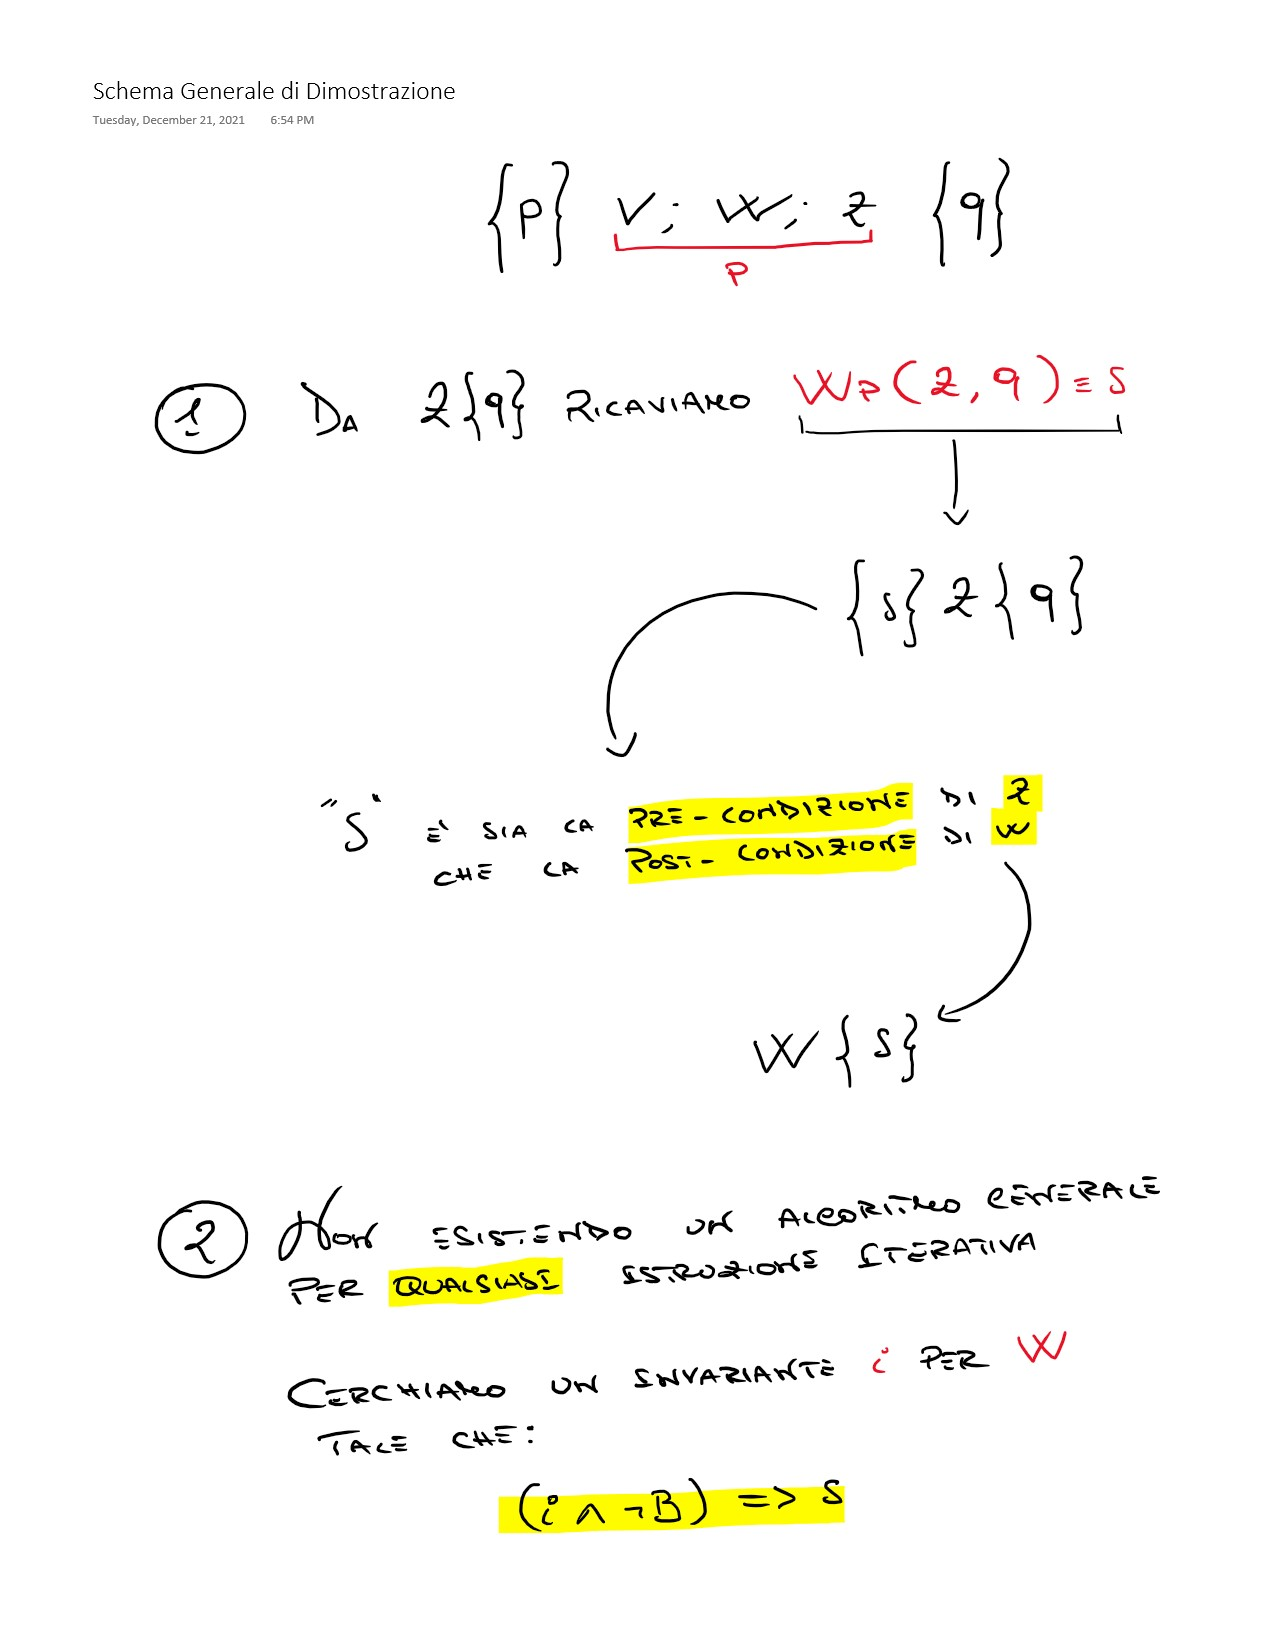
\includepdf[pages=-]{img/SchemaGenerale.pdf}